\chapter{Hybrid parallelization}

% Show, whether there is an advantage of hybrid parallelization compared to pure MPI parallelization. Use up to 4 nodes and use only a new node, if all 48 physical cores are used on the already allocated nodes. 

In this assignment, MPI and OpenMP were combined to investigate the advantages of hybrid parallelization of the heat application. In the previous two chapters, it was found that OpenMP yields higher speedups than MPI when parallelizing within one node, through the efficient use of shared memory, and MPI could be used for communication between nodes. Combining these two programming models could thus yield more scalable results than pure MPI, as then there would be no need for message passing within shared memory regions.

In the implementation, MPI was used for the communication between nodes, and OpenMP for the calculations inside each node. There is one MPI process per node, and all 48 cores of each node are used to create 48 OpenMP threads per node. With a maximum of 4 available nodes, the maximum number of OpenMP threads used was 192, with 4 MPI processes, and the domain could be split into a maximum of 4 areas. At the start of each iteration, the main OpenMP thread waits for the boundaries to be exchanged between MPI processes, and then 48 threads calculate the parallel loop Jacobi relaxation, with a sum reduction for the residual.

Figure \ref{fig:hybrid_speedup} shows the speedups obtained through the hybrid approach. Shown are the results for 2 nodes (96 cores), 3 nodes (144 cores) and 4 nodes (192 cores). The domain was divided in only one dimension at a time as well as for both dimensions. For example, the domain was divided in x in the splits 2x1, 3x1 and 4x1. In the 2D case, only one configuration was possible, which was the 2x2 split.

\begin{figure}[h]
    \centering
    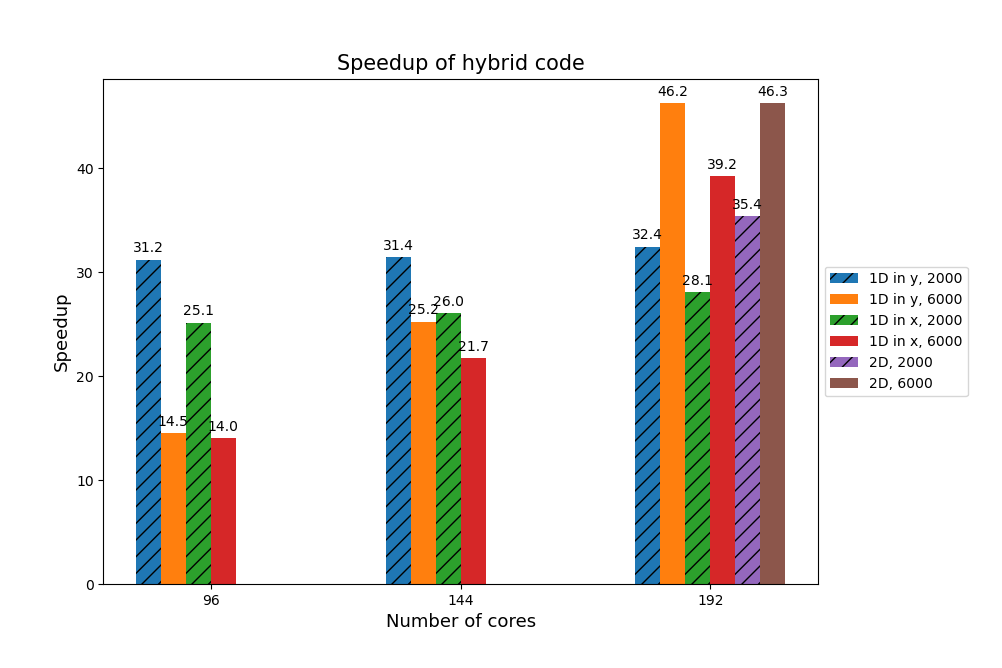
\includegraphics[scale=0.6]{figures/hybrid_speedup.png}
    \caption{Speedups of hybrid implementation.}
    \label{fig:hybrid_speedup}
\end{figure}

As can be seen from the figure, the highest speedups obtained from the hybrid implementation are around 46, which is slightly below the maximum speedups obtained by the pure MPI implementation. This might be due to the fact that the communication between nodes was not threaded, as the main OpenMP thread waits while the MPI processes exchange boundary data. Even though MPI non-blocking communication was used, most threads are thus sleeping while the communication is started.

As with the pure MPI version, there is no clear difference between splitting the domain in only one dimension compared to splitting it in both dimensions. This is likely caused by the same culprit as in the pure MPI version, which, as previously stated, remains unknown. In addition, the higher resolution results in higher speedups, which is consistent with the pure MPI version. 

The results also show that the speedups for resolution 2000 do not scale with increasing number of processors. This could be because the parallelizable code for the smaller resolution is a smaller percentage of the total execution time, and per Amdahl's law is limited to some upper limit. Similar behaviour could be seen in the pure MPI version in figure \ref{fig:speedups-mpi-1d2d}, where the lower resolution's speedup graph starts to taper off reaching its limit at around a speedup of 30.

In conclusion, this assignment showed that this model of hybrid parallelization, where for each node, one MPI process handles communication and OpenMP threads handle the computation, does not present a performance boost when compared to a pure MPI implementation. This can be due to our specific implementation, which already showed some difficulty in the pure MPI version.

